\section{Implementación}

Respecto a la implementación, el software para balancear las clases está implementado en Python mientras que los algoritmos utilizados están implementados en C++.

Como sistema de control de versiones se ha utilizado el software Git, y el código se encuentra alojado y liberado en GitHub \cite{githubProyecto}, bajo una licencia GNU GPLv3 \cite{gplv3}.

Todo el código está documentado utilizando Doxygen \cite{doxygen}, de forma que es posible acceder a la documentación de todas las clases, métodos, funciones y definiciones del código.

\subsection{Preprocesado}

De cara al preprocesado simplemente se han implementado funciones que reciben como entrada los datos y realizan las correspondientes transformaciones, así como funciones para realizar un conteo de clases. También se ha desarrollado un script en Python que será el encargado de realizar el sobremuestreo de datos para las clases minoritarias, como se comento en la sección del preprocesado de datos.

\subsection{Algoritmos}

Con respecto a la implementación de los algoritmos utilizados, estos se han implementado en C++.

La implementación tiene un enfoque orientado a objetos, además de ciertas funciones auxiliares que utilizaremos a lo largo de la implementación. De cara a implementar las distintas clases necesarias así como las funciones se ha encapsulado todo en un espacio de nombres de C++ que se llamará \texttt{algoritmos\_poblacion\_expresiones}. Esto nos evitará problemas de definiciones si en un futuro se utiliza el software para otros proyectos, además de dar una mejor estructura del código.

\subsubsection{Clase AlgoritmoPoblacion}

El código esta estructurado utilizando herencia y plantillas de C++, de forma que nos encontramos con una clase \texttt{AlgoritmoPoblacion<T>}, que tiene como plantilla la clase de expresión que utilizará dicho algoritmo. Esta clase será abstracta, y nunca se podrá utilizar por si misma.

Esta clase contendrá los datos y métodos comunes a cualquier algoritmo que utilice una población, de forma que las operaciones comunes estén definidas y no sea necesario repetir código si necesitamos hacer distintas variaciones. De cara a implementar un algoritmo simplemente se ha de crear una clase que derive de esta e implemente un método \texttt{ajustar}, que será el que se encargue de ajustar dicho algoritmo concreto, además de todo lo que se considere oportuno.

\begin{figure}[H]
	 \centering
	 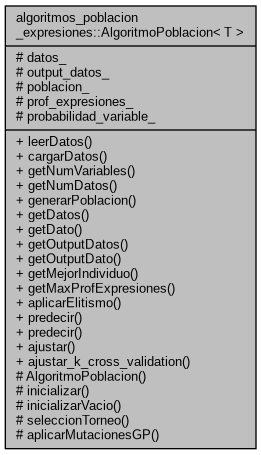
\includegraphics[width=0.2\textwidth]{clases/algoritmo_poblacion.png}
	 \caption{Diagrama de la clase AlgoritmoPoblacion.}
	\label{fig:diagrama_clase_algoritmo_poblacion}
\end{figure}


\subsubsection{Clase Poblacion}

La clase \texttt{AlgoritmoPoblacion<T>} contiene una población, la cual será un conjunto de datos de tipo \texttt{T}, que puede realizar ciertas operaciones concretas, en este caso encapsularemos dichas operaciones y atributos en la clase \texttt{Poblacion<T>}.

Estas clase se tratará de una clase de consulta de cara a almacenar todos los individuos que entran en juego en nuestros algoritmos, así como una forma de aplicar ciertas operaciones a todos los individuos, como por ejemplo evaluarlos.

\begin{figure}[H]
	 \centering
	 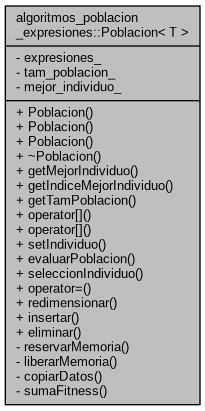
\includegraphics[width=0.2\textwidth]{clases/poblacion.png}
	 \caption{Diagrama de la clase Poblacion.}
	\label{fig:diagrama_clase_poblacion}
\end{figure}

\newpage

\subsubsection{Clase Expresion y clase Nodo}

Una vez tenemos la parte genérica de un algoritmo con una población de expresiones, necesitamos una estructura que nos represente dichas expresiones, en este caso, la clase \texttt{Expresion}. Esta clase será la expresión original de Programación Genética, que contendrá un árbol que conformará la expresión. Este árbol se ha representado como un vector con la representación en preorder del árbol.

En esta clase encontraremos como atributos el propio árbol, el ajuste de dicha expresión, la longitud máxima que permitiremos que tenga la expresión, entre otros atributos auxiliares. También podemos encontrar como métodos distintas operaciones de las expresiones de Programación Genética, como intercambiar un subárbol, evaluar la expresión con ciertos datos, entre otras.

Dichos árboles serán un conjunto de nodos, el cual representaremos con la clase \texttt{Nodo}. Cada nodo podrá ser de un tipo distinto y nosotros utilizaremos los siguientes tipos:

\begin{itemize}
	\item Variable: Indica que el nodo se refiere a una variable del conjunto de datos de entrada.
	\item Número: El nodo será una constante numérica.
	\item Más: Operador de suma.
	\item Menos: Operador de resta.
	\item Por: Operador de multiplicación.
	\item Entre: Operador de división.
\end{itemize}

Hemos escogido pocos operadores de cara a mantener las expresiones resultantes simples.

\begin{figure}[H]
	 \centering
	 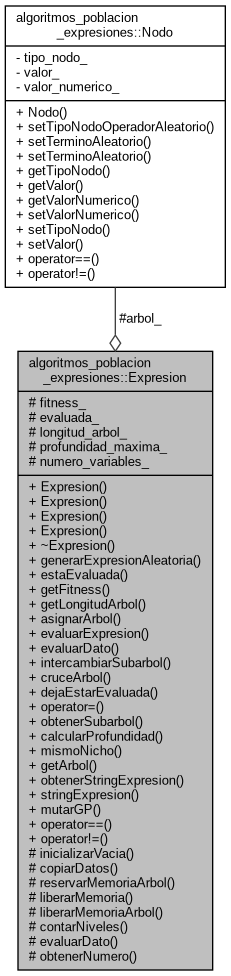
\includegraphics[width=0.2\textwidth]{clases/expresion_nodo.png}
	 \caption{Diagrama de las clases Expresion y Nodo.}
	\label{fig:diagrama_clase_expresion_nodo}
\end{figure}

\newpage

\subsubsection{Clase AlgoritmoPG}

Esta clase se trata de la clase del algoritmo de Programación Genética que implementamos. Esta clase \texttt{AlgoritmoPG} será una clase hija de \texttt{AlgoritmoPoblacion<Expresion>}, es decir, el algoritmo de Programación Genética es un algoritmo con una población de \texttt{Expresion}.

\texttt{AlgoritmoPG} simplemente implementa el método \texttt{ajustar}, que será la forma en la que el algoritmo se ajuste para los datos y etiquetas dados.


\begin{figure}[H]
	 \centering
	 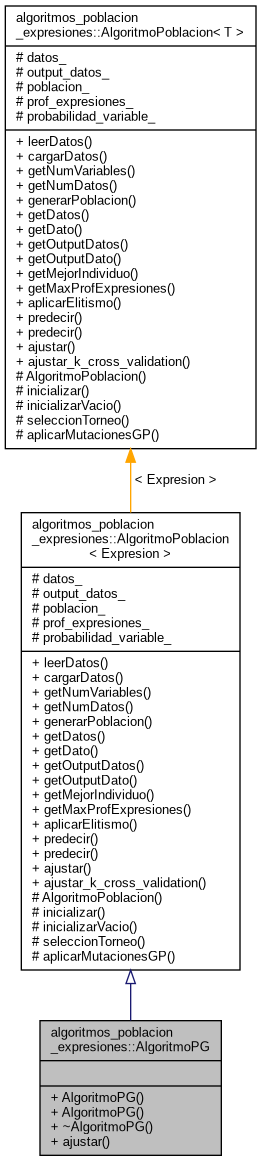
\includegraphics[width=0.2\textwidth]{clases/algoritmoPG.png}
	 \caption{Diagrama de la clase AlgoritmoPG.}
	\label{fig:diagrama_clase_algoritmoPG}
\end{figure}

\newpage

\subsubsection{Clase Expresion\_GAP y AlgoritmoGAP}

Como vemos, con la estructura de clases con plantillas introducir un nuevo algoritmo es tan simple como definir el comportamiento de la expresión a utilizar y como se ajusta dicho algoritmo a los datos. Por este motivo, introducir la variante de GA-P es muy simple.

Para las expresiones de GA-P usaremos como base las expresiones de Programación Genética, ya que el único añadido es el cromosoma, y la forma en la que se obtienen los valores numéricos, por lo tanto la clase \texttt{Expresion\_GAP} quedará de la siguiente forma.



\begin{figure}[H]
    \centering
	 \begin{subfigure}[b]{0.49\textwidth}
		 \centering
		 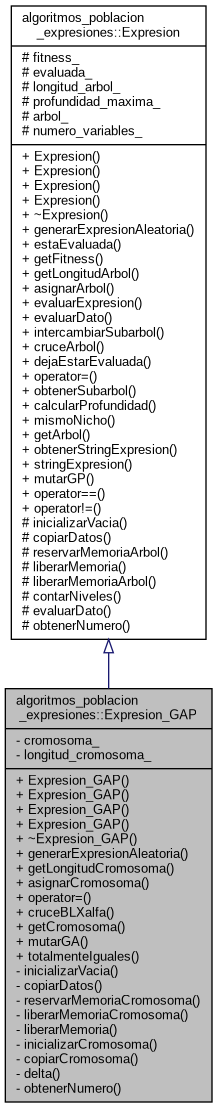
\includegraphics[width=0.3\textwidth]{clases/expresion_gap.png}
		 \caption{Diagrama de la clase Expresion\_GAP.}
		\label{fig:diagrama_clase_expresion_gap}
	 \end{subfigure}
	\begin{subfigure}[b]{0.49\textwidth}
		 \centering
		 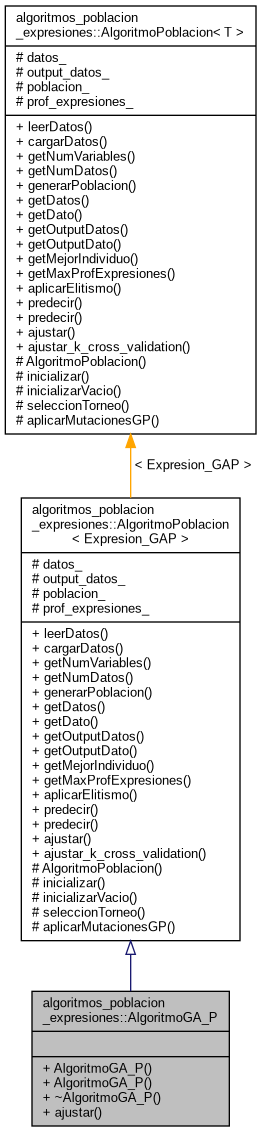
\includegraphics[width=0.3\textwidth]{clases/algoritmo_gap.png}
 		\caption{Diagrama de la clase Algoritmo\_GAP.}
 	  \label{fig:diagrama_clase_algoritmo_gap}
   \end{subfigure}

	\caption{Diagrama de clases de Algoritmo\_GAP y Expresion\_GAP.}
	\label{fig:diagrama_clases_gap}
\end{figure}


\subsubsection{Clase Parametros}

De cara a hacer más sencillo el uso de los algoritmos también se ha implementado una clase \texttt{Parametros} que contiene todos los parámetros posibles para los algoritmos. De esta forma gestionar los parámetros con los que se lanza un algoritmo es mucho más sencillo, además de que nos permite una mayor flexibilidad a la hora de realizar distintas ejecuciones.

\begin{figure}[H]
	 \centering
	 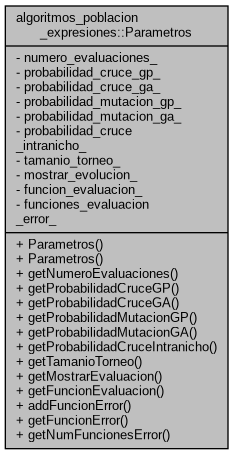
\includegraphics[width=0.2\textwidth]{clases/parametros.png}
	 \caption{Diagrama de la clase AlgoritmoPG.}
	\label{fig:diagrama_clase_algoritmoPG}
\end{figure}


\subsubsection{Diagrama de clases final}

Con todas estas clases, el diagrama final quedaría de la siguiente forma:

\begin{figure}[H]
	 \centering
	 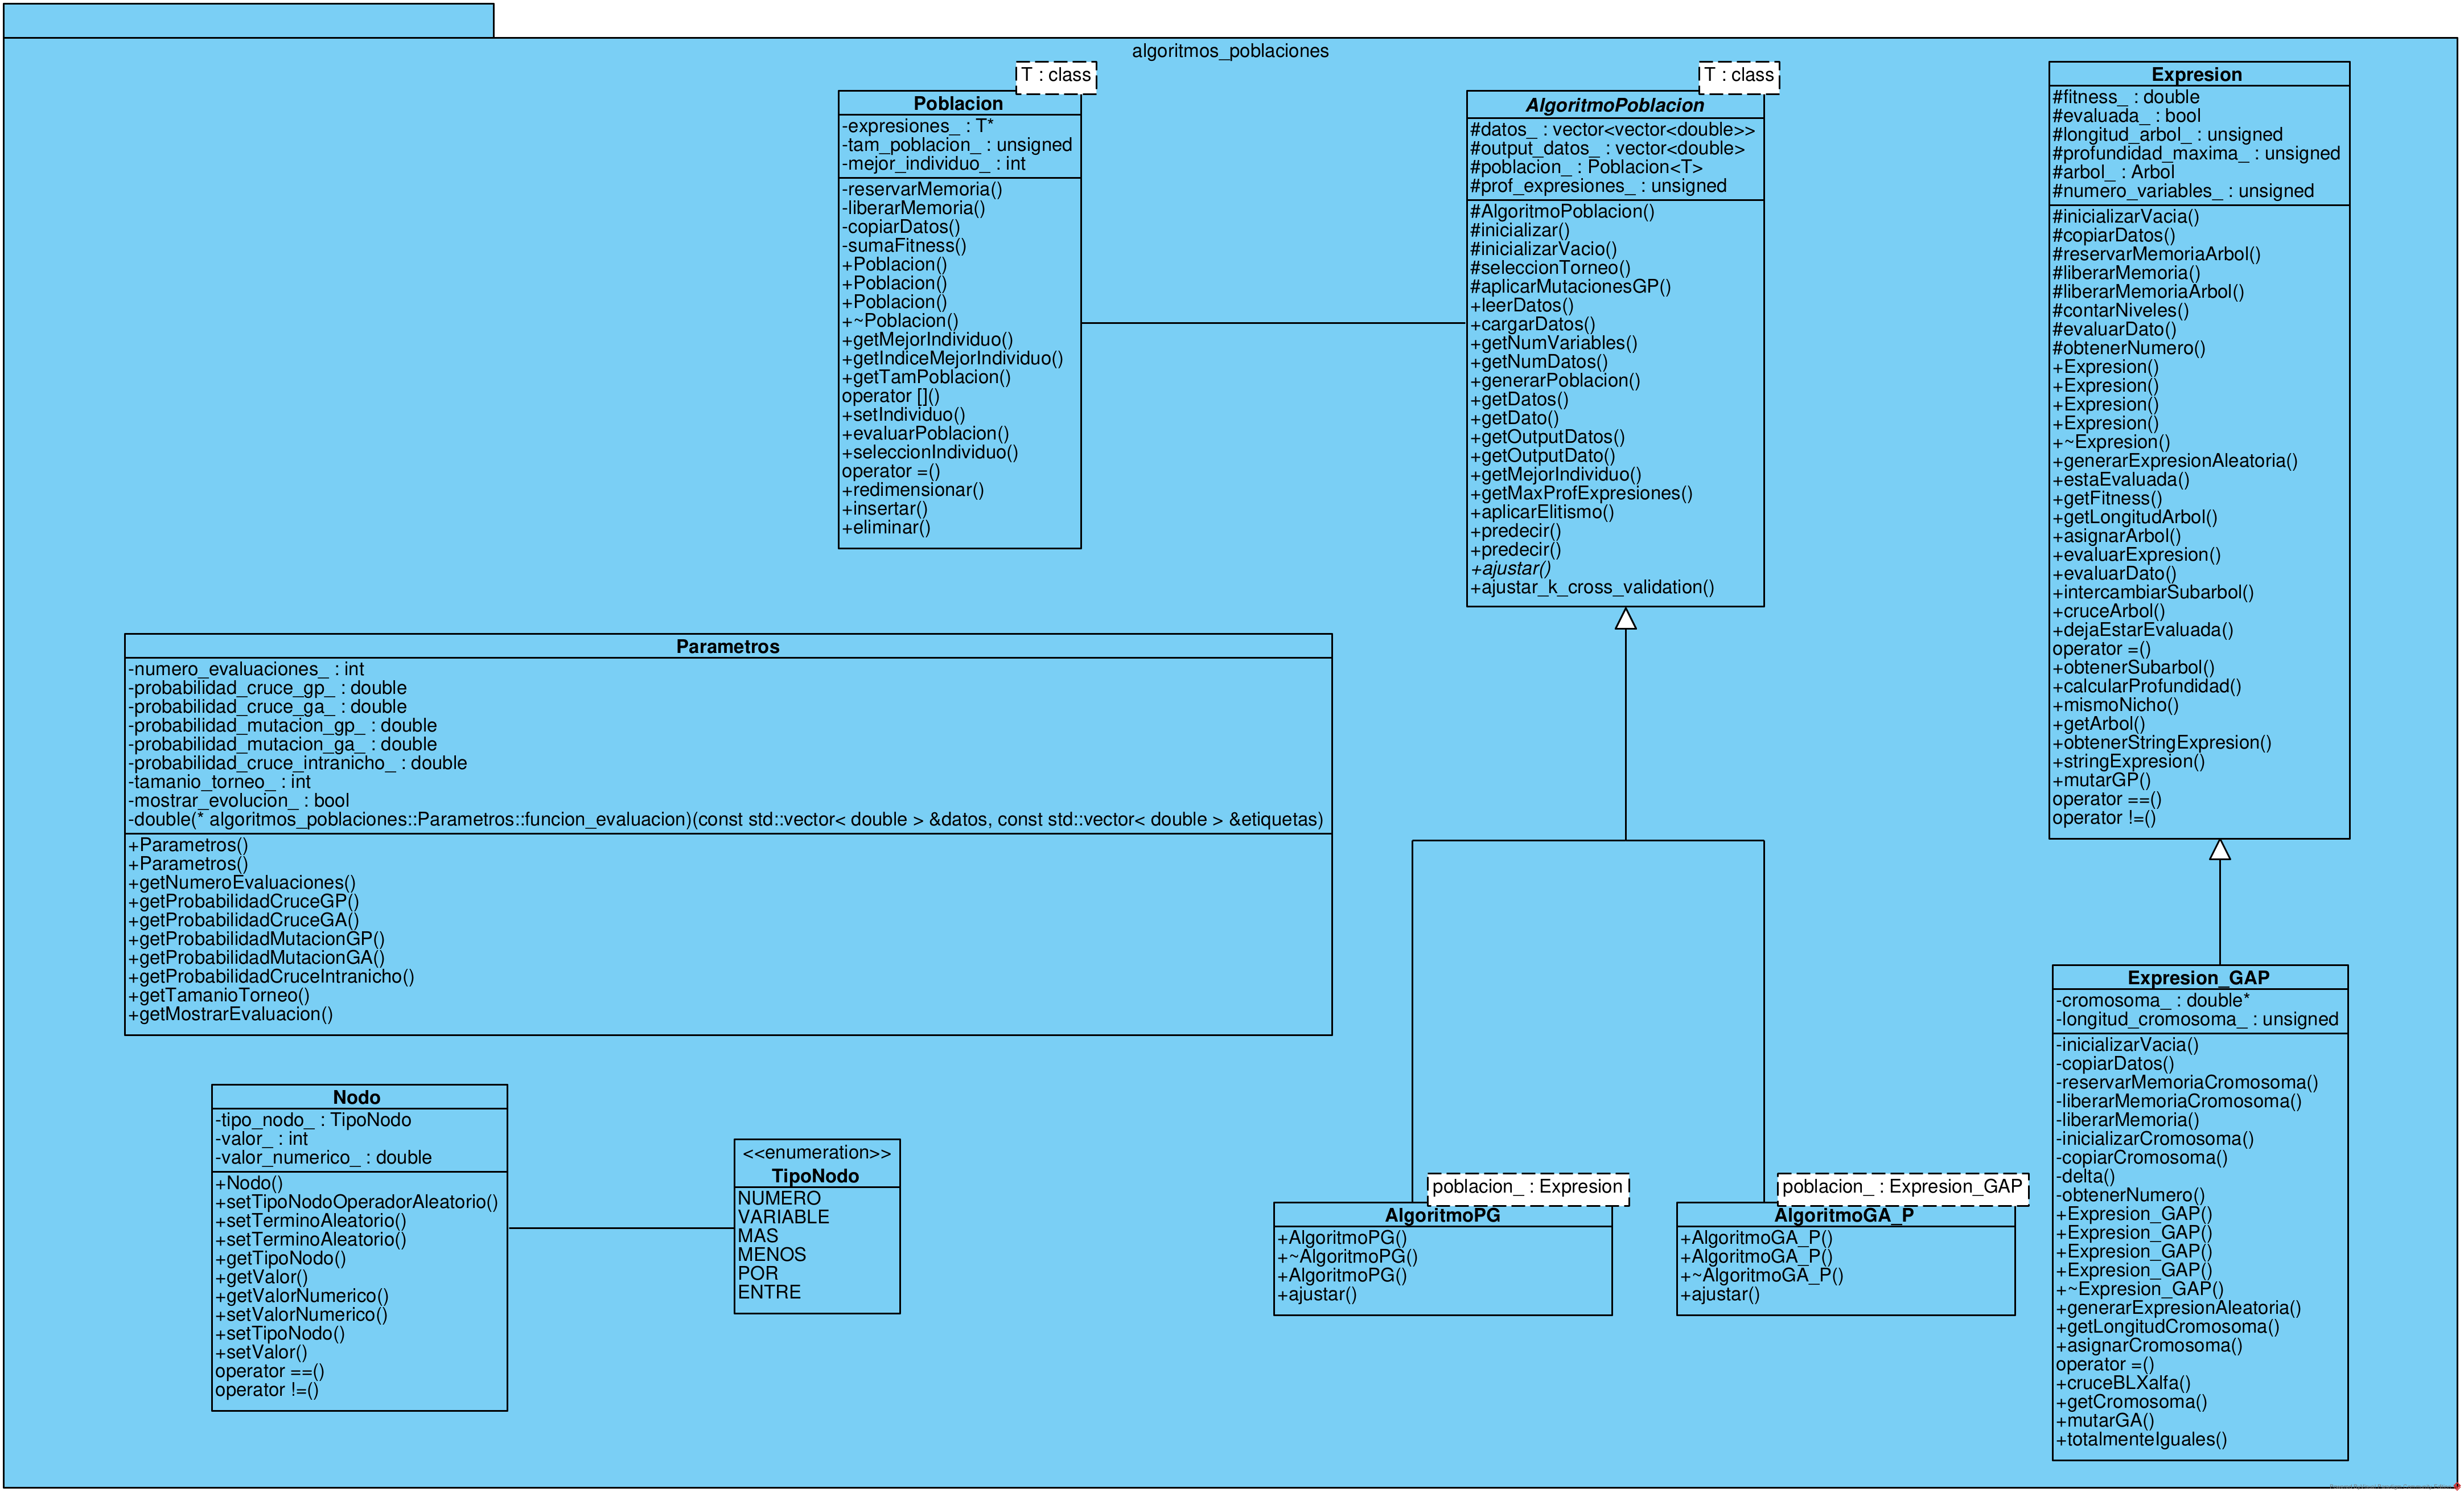
\includegraphics[width=\textwidth]{diagrama_clases.png}
	 \caption{Diagrama de clases.}
	\label{fig:diagrama_clases}
\end{figure}

Cabe destacar algunas declaraciones de tipos internas que se han hecho, como la del tipo \texttt{Arbol}, que es el tipo \texttt{Nodo *} (puntero a un nodo), o la del tipo \texttt{funcion\_evaluacion\_t}, que se trata de un puntero a una función que recibe una matriz de datos y un vector de etiquetas y devuelve un real. Esta función será la función que utilicemos para evaluar las expresiones, pero debido a su complejidad sintáctica se ha definido este tipo para que nombrarlo sea más fácil. El tipo completo sería:

\begin{lstlisting}[language=C++]
double (*funcion_evaluacion_t)(const std::vector<double> & datos, const std::vector<double> & etiquetas)
\end{lstlisting}

\subsubsection{Otras funciones auxiliares}

También disponemos de algunas funciones auxiliares, que nos servirán a lo largo de todo el código, como la comprobación de si dos valores reales son iguales teniendo en cuenta los problemas de representación de números en coma flotante de C++, o distintas posibles funciones de evaluación que hemos predefinido.




\subsection{Uso de paralelismo}
